\section{Changing Motion\footnote{
1990-93 Dept. of Physics and Astronomy, Dickinson College. Supported by FIPSE
(U.S. Dept. of Ed.) and NSF. Portions of this material may have been modified
locally and may not have been classroom tested at Dickinson College.
}}
\label{changing_motion}

\makelabheader %(Space for student name, etc., defined in master.tex or labmanual_formatting_commands.tex)

\bigskip
\textbf{Objectives} 
\vspace{-\parskip}
\begin{itemize}
\item To learn how to relate graphs of acceleration \textit{vs.}~time to the motions they represent. 
\item To understand the relationship between position \textit{vs.}~time, velocity \textit{vs.}~time,
and acceleration \textit{vs.}~time graphs.
\end{itemize}

\textbf{Introduction: Velocity and Acceleration Graphs} 

We are interested in having you learn to describe simple motions in which the
velocity of an object is changing. In order to learn to describe motion in more
detail for some simple situations, you will be asked to observe and describe
the motion of a dynamics cart on a track. Although graphs and words are still
important representations of these motions, you will also be asked to draw velocity
vectors, arrows that indicate both the direction and speed of a moving object.
Thus, you will also learn how to represent simple motions with velocity diagrams.

In the last session, you looked at position \textit{vs.}~time and velocity \textit{vs.}~time graphs
of the motion of your body as you moved at a ``constant'' velocity.
The data for the graphs were collected using a motion detector. Your goal in
this session is to learn how to describe various kinds of motion in more detail.
It is not enough when studying motion in physics to simply say that ``the
object is moving toward the right'' or ``it is standing still.''
You have probably realized that a velocity \textit{vs.}~time graph is better than a position
vs. time graph when you want to know how fast and in what direction you are
moving at each instant in time as you walk. When the velocity of an object is
changing, it is also important to know how it is changing. The rate of change
of velocity is known as the acceleration. 

In order to get a feeling for acceleration, it is helpful to create and learn
to interpret velocity \textit{vs.}~time and acceleration \textit{vs.}~time graphs for some relatively
simple motions of a cart on a track. You will be observing the cart with the
motion detector as it moves at a constant velocity and as it changes its velocity
at a constant rate. Use the 
\filename{P\_V\_A\_Graphs.cap} program in the \filename{\coursefolder} folder
for all of the activities in this unit.

\bigskip
\textbf{Apparatus} 
\vspace{-\parskip}
\begin{itemize}
\item Pasco 550 Interface
\item Ultrasonic motion detector 
\item \textit{Capstone} software (\filename{P\_V\_A\_Graphs.cap} experiment file)
\item Collision cart and track 
\item Lab stand to incline the track 
\end{itemize}

\textbf{Activity 1: Graphs of Constant Velocity} 

Let's start by giving the cart a push along the level track and graphing its
motion. 

(a) Based on your observations of the motions of your body in the last session,
how should the position and velocity graphs look if you move the cart at a constant
velocity away from the motion detector starting at the 0.5 meter mark? Sketch
your predictions with dashed lines on the axes that follow.

%\vspace{-0.1in}
{\par\centering 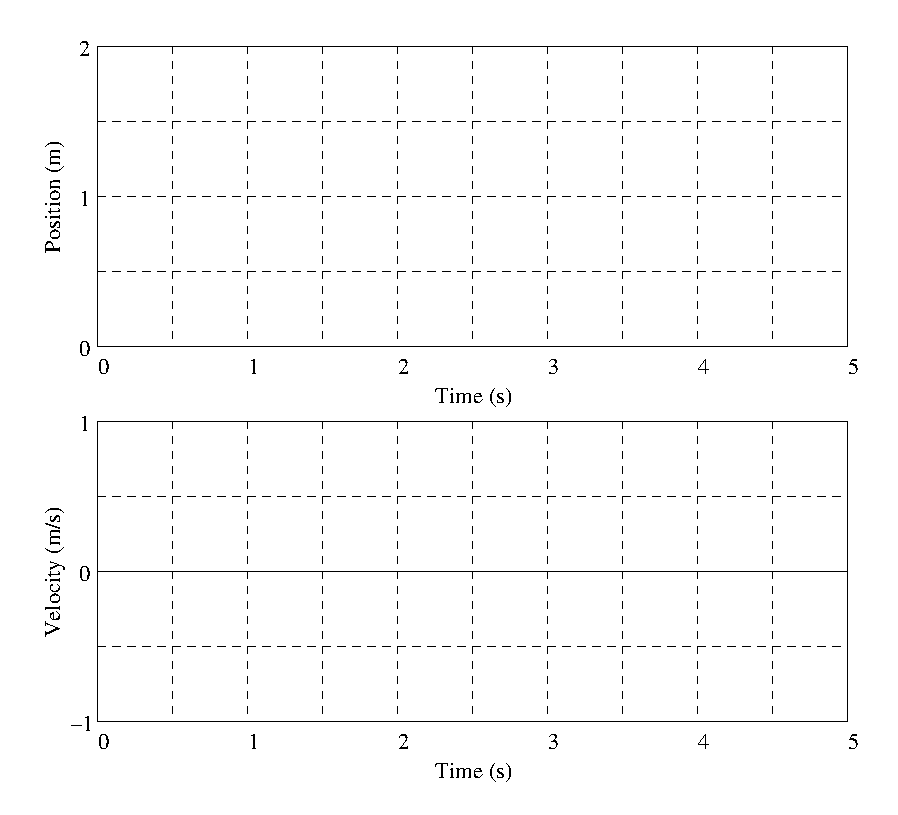
\includegraphics[scale=1]{changing/changing_fig1.eps} \par}
\vspace{-0.1in}

(b) Acceleration is defined as the time rate of change of velocity. Sketch your
prediction of the cart acceleration on the axes that follow using a dashed line.

%\vspace{-0.1in}
{\par\centering 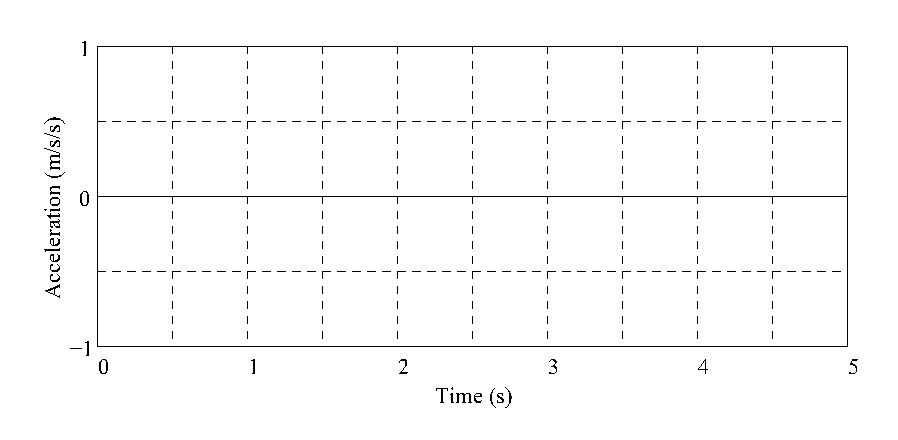
\includegraphics[scale=1]{changing/changing_fig2.eps} \par}
%\vspace{-0.1in}

(c) Test your prediction. Be sure that the cart is never closer than 0.15 meter
from the motion detector. Try several times until you get a fairly constant
velocity. Sketch your results with solid lines on the axes shown above. The
acceleration \textit{vs.}~time graphs will exhibit small fluctuations due to irregularities
in the motion of the cart. You should ignore these fluctuations and draw smooth
patterns.

\pagebreak[2]
(d) Did your graphs agree with your predictions? What characterizes constant
velocity motion on a position \textit{vs.}~time graph? 
\answerspace{10mm}

(e) What characterizes constant velocity motion on a velocity \textit{vs.}~time graph?
\answerspace{10mm}

(f) What characterizes constant velocity motion on an acceleration \textit{vs.}~time graph?
\answerspace{10mm}

%\textbf{Finding Accelerations} 
\textbf{Activity 2: Representing Acceleration} 

To find the average acceleration of the cart during some time interval (the
average time rate of change of its velocity), you must measure its velocity
at two different times, calculate the difference between the final value and
the initial value and divide by the time interval.

To find the acceleration vector from two velocity vectors, you must first find
the vector representing the change in velocity by subtracting the initial velocity
vector from the final one. Then you divide this vector by the time interval. 


(a) Calculate the average acceleration during some time interval from your velocity graph in Activity 1.  Does the result agree with your acceleration graph in Activity 1?
\answerspace{20mm}

(b) The diagram below shows the positions of the cart at equal time intervals.
(This is like taking snapshots of the cart at equal time intervals.) At each
indicated time, sketch, and label, a vector above the cart which might represent the velocity
of the cart at that time while it is moving at a constant velocity away from
the motion detector.

%\vspace{0.3cm}
%{\par\centering 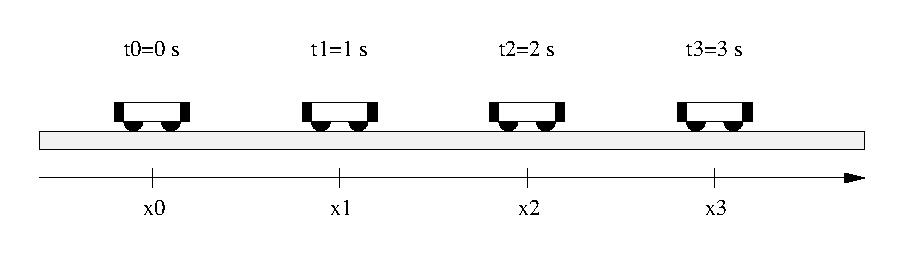
\includegraphics{changing/changing_fig3.eps} \par}
{\par\centering 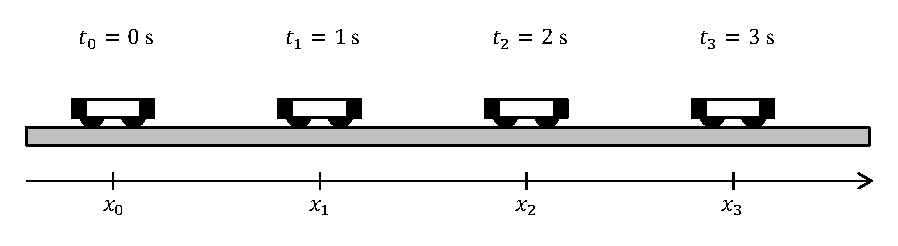
\includegraphics{changing/carts_const_v.eps} \par}
%\vspace{0.3cm}

(c) Show how you would find the vector representing the change in velocity
between the times 1.0 s and 2.0 s by creating a vector diagram using the 
vectors above. From the resultant vector, what value would you calculate for 
the acceleration? Is this value in agreement
with the acceleration graph you obtained in Activity 1?
\answerspace{20mm}

\pagebreak[2]
%\textbf{Speeding Up at a Moderate Rate} 
\textbf{Activity 3: Graphs Depicting Speeding Up} 

In this activity you will look at velocity and acceleration graphs of the
motion of a cart when its velocity is changing. You will be able to see how
these two representations of the motion are related to each other when the cart
is speeding up.

In order to get your cart speeding up smoothly \textit{use the lab stand to raise the
track several centimeters at the end where the motion detector is mounted}.

(a) Predict the shape of the position, velocity, and acceleration \textit{vs.}~time graphs
for the cart moving away from the sensor and speeding up. Sketch your predictions
on the following axes using dashed lines.

\vspace{-0.2cm}
{\par\centering 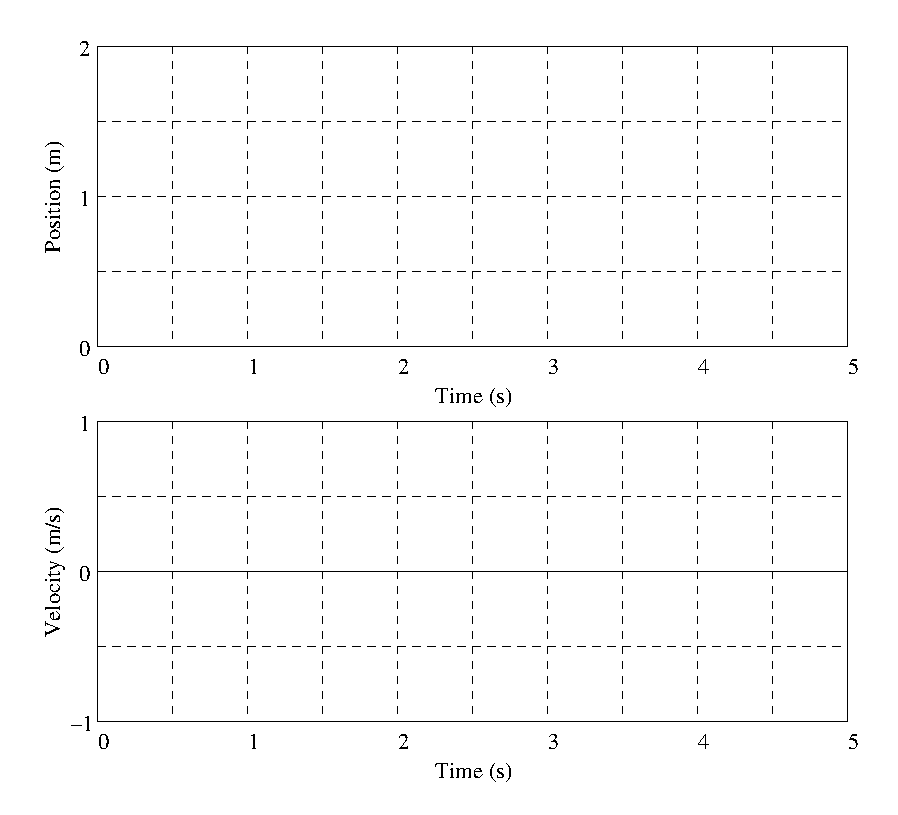
\includegraphics[scale=0.93]{changing/changing_fig1.eps} \par}
%\vspace{0.3cm}

\vspace{-0.4cm}
{\par\centering 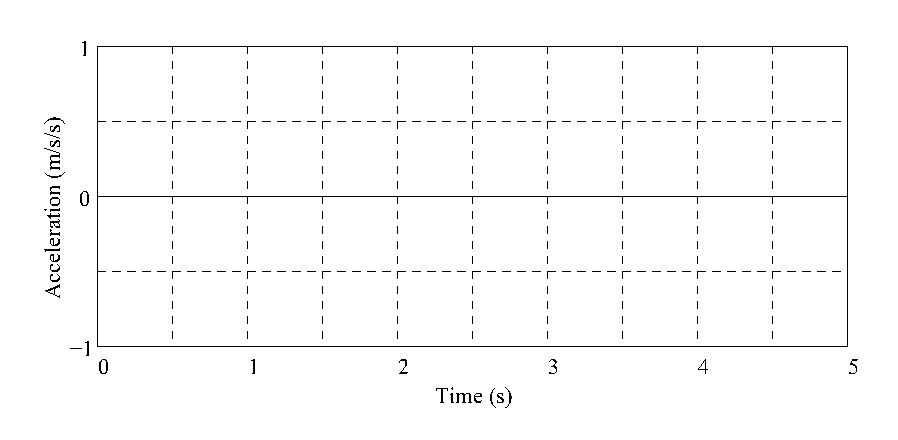
\includegraphics[scale=0.93,trim={0 0 0 0.4cm},clip]{changing/changing_fig2.eps} \par}
%\vspace{0.3cm}

(b) Create graphs of the motion of your cart as it moves away from the detector
and speeds up. Sketch the graphs neatly on the above axes using solid lines.

\pagebreak[2]
(c) How does your position graph differ from the position graphs for steady
(constant velocity) motion? 
\vspace{13mm}

(d) What feature of your velocity graph signifies that the motion was away from
the detector? 
\vspace{13mm}

(e) What feature of your velocity graph signifies that the cart was speeding
up? How would a graph of motion with a constant velocity differ? 
\vspace{13mm}

(f) During the time that the cart is speeding up, is the acceleration positive
or negative? How does speeding up while moving away from the detector result
in this sign of acceleration? Hint: Remember that acceleration is the rate of
change of velocity. Look at how the velocity is changing. 
\vspace{13mm}

(g) How does the velocity vary in time as the cart speeds up? Does it increase
at a steady rate or in some other way? 
\vspace{13mm}

(h) How does the acceleration vary in time as the cart speeds up? Is this what
you expect based on the velocity graph? Explain.
\vspace{13mm}

(i) Do not delete the graphs from the computer screen.  They will be used in Activity 5.
\vspace{10mm}

\textbf{Activity 4: Using Vectors to Describe Acceleration} 

Let's return to the Vector Diagram representation and use it to describe the
acceleration.

(a) The diagram that follows shows the positions of the cart at equal time intervals.
At each indicated time, sketch, and label, a vector above the cart which might represent
the velocity of the cart at that time while it is moving away from the motion
detector and speeding up.

\vspace{0.3cm}
%{\par\centering 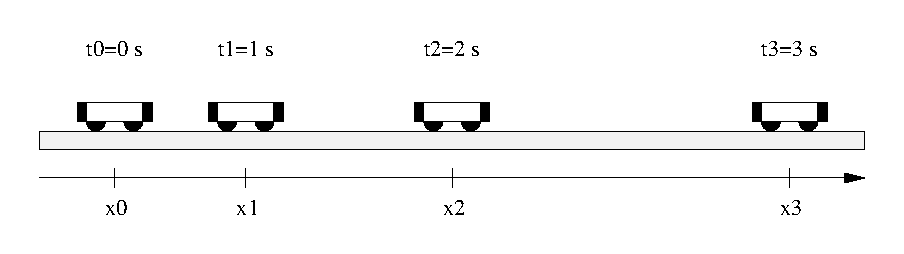
\includegraphics{changing/changing_fig4.eps} \par}
{\par\centering 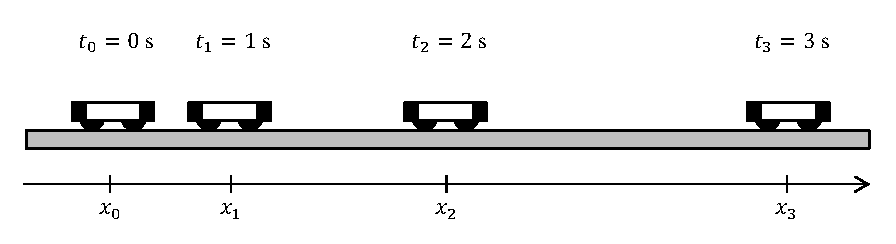
\includegraphics{changing/carts_const_a.eps} \par}
\vspace{0.3cm}

(b) Show below how you would find the approximate length and direction of the
vector representing the change in velocity between the times 1.0 s and 2.0 s
by creating a vector diagram using the vectors above. No quantitative 
calculations are needed. Based on the direction of the resultant vector and 
the direction of the positive x-axis, what is the sign of the acceleration? 
Does this agree with your answer to Activity 3 (f)?
\answerspace{20mm}

%\textbf{Measuring Acceleration }
\textbf{Activity 5: Measuring and Calculating Accelerations}

In this investigation you will analyze the motion of your accelerated cart quantitatively.
This analysis will be quantitative in the sense that your results will consist
of numbers. You will determine the cart's acceleration from the slope of your
velocity \textit{vs.}~time graph and compare it to the average acceleration read from
the acceleration \textit{vs.}~time graph. 

(a) Using the \textbf{Statistics} function on your acceleration graph from Activity 3, determine the average acceleration and the standard deviation by selecting only values from the portion of the graph after the cart was released and before you stopped it. See \textbf{Appendix \ref{capstone}: Capstone} for information on how to use the \textbf{Statistics} function. Record these values here:
\answerspace{20mm}

(b) Write the acceleration with its uncertainty (the standard deviation) here:
\answerspace{20mm}

(c) The average acceleration during a particular time period is defined as the
change in velocity divided by the change in time. This is the average rate of
change of velocity. By definition, the rate of change of a quantity graphed
with respect to time is also the slope of the curve. Thus the (average) slope
of an object's velocity \textit{vs.}~time graph is the (average) acceleration of the
object.

Select the velocity vs. time graph from Activity 3 and open the \textbf{Delta Tool} function on the graph menu bar. Determine quantities \( \Delta v\) and \( \Delta t\) for two points on the velocity graph using the Delta Tool, 
in the same way that you did on the position vs. time graph in the previous experiment. Record the values of 
\( \Delta v\) and \( \Delta t\) here:
\answerspace{20mm}

(d) Divide the change in velocity by the change in time. This is the average acceleration. Show your calculation here:
\answerspace{20mm}

\pagebreak[2]
(e) Is the acceleration positive or negative? Is this what you expected? 
\answerspace{15mm}

(f) Does the average acceleration you just calculated agree with the average
acceleration you calculated from the acceleration \textit{vs.}~time graph? Do you expect them to agree? How would you account for any differences? 
\answerspace{20mm}

\textbf{Activity 6: Speeding Up at a Faster Rate} 

(a) Suppose that you accelerate your cart at a faster rate by raising the end of the track several more centimeters. How would your velocity and acceleration graphs change? 
\answerspace{15mm}

(b) Resketch the velocity and acceleration graphs you found in Activity 3 using
the axes that follow.

\vspace{-0.3cm}
{\par\centering 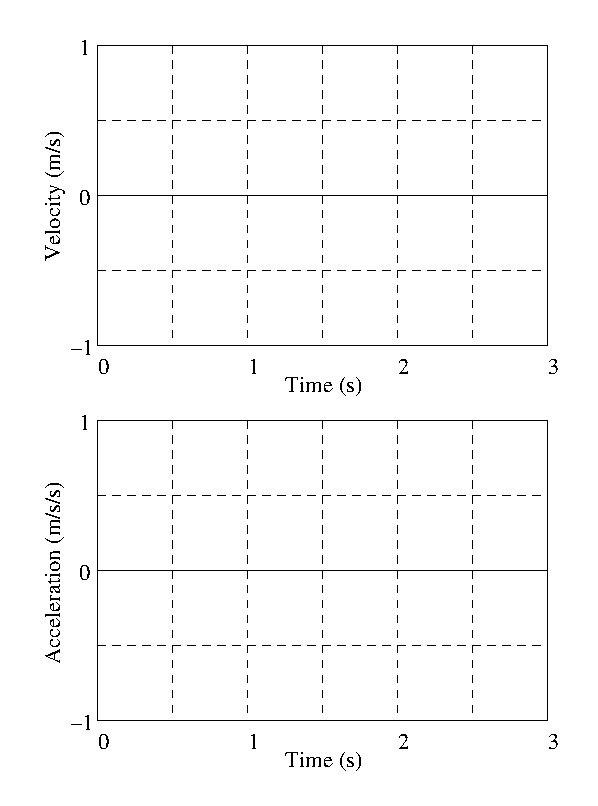
\includegraphics{changing/changing_fig5.eps} \par}
\vspace{-0.3cm}

(c) In the previous set of axes, use a dashed line or another color to sketch
your predictions for the general graphs that depict a cart speeding up at a
faster rate. Exact predictions are not expected. We just want to know how you
think the general shapes of the graphs will change.

\pagebreak[2]
(d) Test your predictions by accelerating the cart with the end of the track raised several centimeters more than in Activity 3. Repeat if necessary to get nice graphs and then sketch the results using the axes that follow.

%\vspace{0.3cm}
{\par\centering 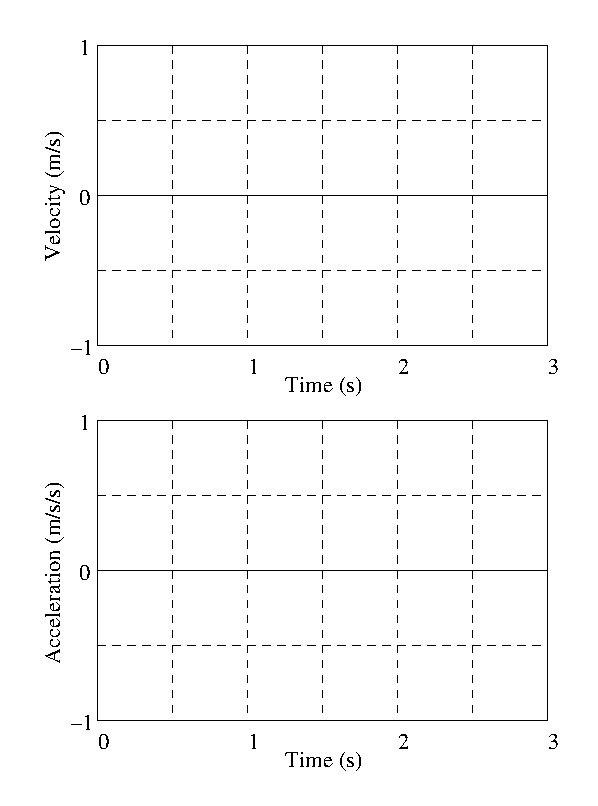
\includegraphics{changing/changing_fig5.eps} \par}
%\vspace{0.3cm}

(e) Did the general shapes of your velocity and acceleration graphs agree with
your predictions? How is the greater magnitude (size) of acceleration represented
on a velocity \textit{vs.}~time graph? 
\answerspace{25mm}

(f) How is the greater magnitude (size) of acceleration represented on an acceleration
vs. time graph? 
\answerspace{25mm}

\pagebreak[2]
\textbf{Homework} 

1. An object moving along a line (the + position axis) has the acceleration-time
graph shown below. Describe how might the object move to create this graph if
it is moving away from the origin?

\vspace{0.3cm}
{\par \centering 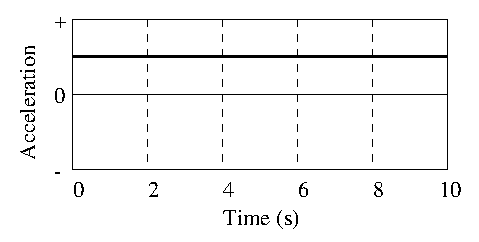
\includegraphics{changing/changing_fig6.eps} \par}
\answerspace{1.5cm}

2. Sketch on the axes below a velocity-time graph that goes with the above acceleration-time
graph.

\vspace{0.3cm}
{\par\centering 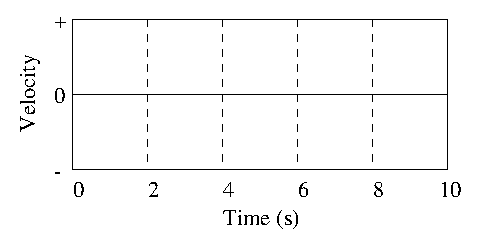
\includegraphics{changing/changing_fig7.eps} \par}
%\answerspace{1.0cm}
\vspace{0.4cm}

3. For each of the velocity-time graphs below, sketch the shape of the acceleration-time
graph that goes with it.

\vspace{0.3cm}
{\par\centering 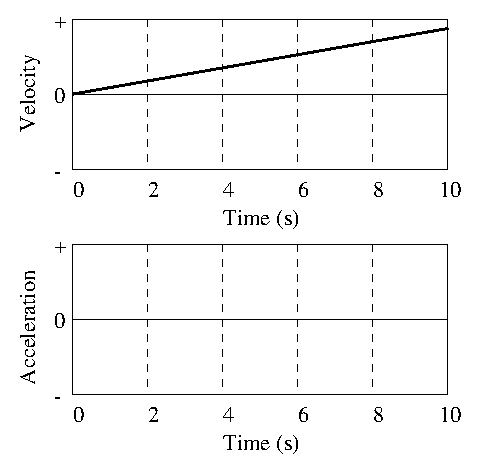
\includegraphics{changing/changing_fig8.eps} \par}
\vspace{0.3cm}

\vspace{0.3cm}
{\par\centering 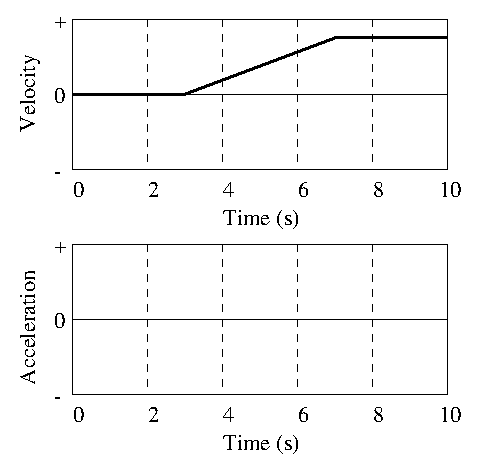
\includegraphics{changing/changing_fig9.eps} \par}
\vspace{0.3cm}

4. The following is a velocity-time graph for a car.

\vspace{0.3cm}
{\par\centering 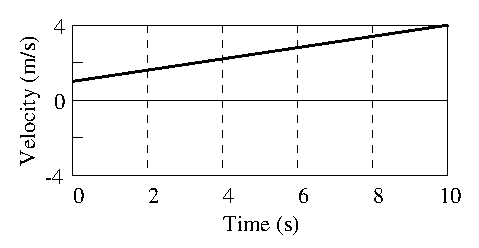
\includegraphics{changing/changing_fig10.eps} \par}
\vspace{0.3cm}

What is the average acceleration of the car? Show your work below.
\answerspace{30mm}

5. Which position-time graph below could be that for a cart that is steadily
accelerating away from the origin?

\vspace{0.3cm}
{\par\centering 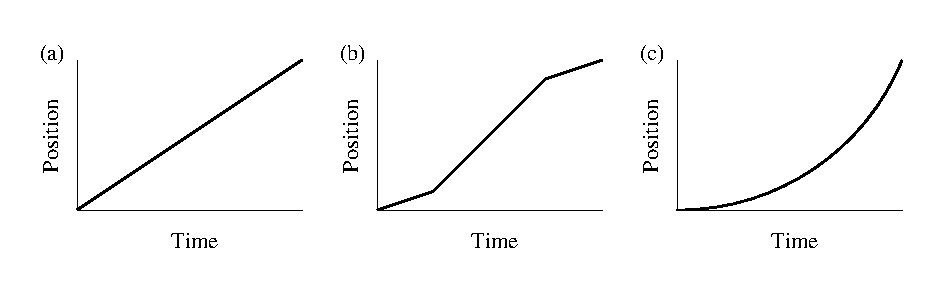
\includegraphics{changing/changing_fig11.eps} \par}
\vspace{0.3cm}

\pagebreak[2]
A car can move along a line (the + position axis). Sketch velocity-time and
acceleration-time graphs which correspond to each of the following descriptions
of the car's motion.

6. The car starts from rest and moves away from the origin increasing its speed
at a steady rate.

\vspace{0.3cm}
{\par\centering 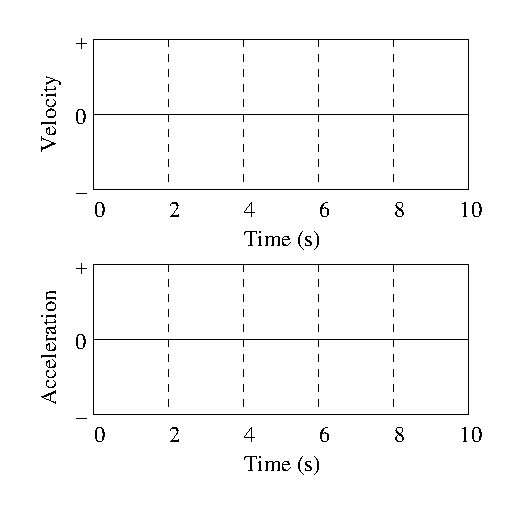
\includegraphics[width=0.55\textwidth]{changing/changing_fig12.eps} \par}
\answerspace{0.3cm}

7. The car is moving away from the origin at a constant velocity.

\vspace{0.3cm}
{\par\centering 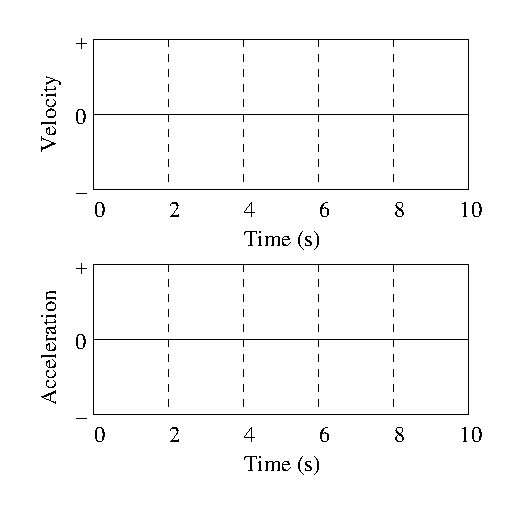
\includegraphics[width=0.55\textwidth]{changing/changing_fig12.eps} \par}
\answerspace{0.3cm}

%\pagebreak[2]
\newpage
8. The car starts from rest and moves away from the origin increasing its speed
at a steady rate twice as large as in (6) above.

\vspace{0.3cm}
{\par\centering 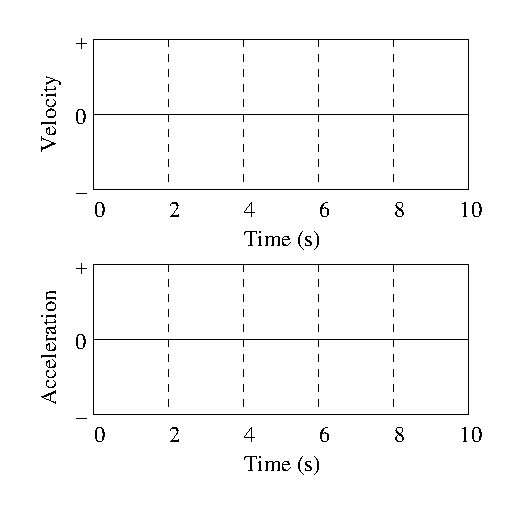
\includegraphics[width=0.55\textwidth]{changing/changing_fig12.eps} \par}
\vspace{0.3cm}

9. The car is moving away from the origin at a constant velocity twice as large
as in (7) above.

\vspace{0.3cm}
{\par\centering 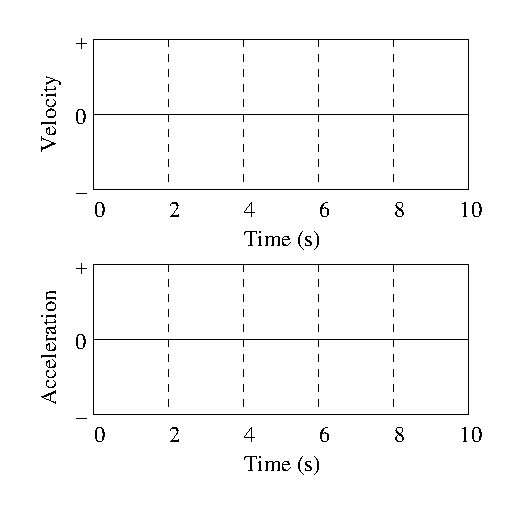
\includegraphics[width=0.55\textwidth]{changing/changing_fig12.eps} \par}
\vspace{0.3cm}

